\documentclass[
   aspectratio=169, % default is 43
   10pt, % font size, default is 11pt
   nosectionframes,
   uniqueslidenumber,
   % handout,
   professionalfonts
]{beamer}

\usepackage[T1]{fontenc}
\usepackage[utf8]{inputenc}
\usepackage[sfdefault]{FiraSans}

\usepackage{stmaryrd}
\usepackage[vvarbb]{notomath}
\usepackage{FiraMono}
\usepackage{tikz,forest}
\usepackage{fontawesome}
\usepackage{../abstract-interpretation-ltx/absint}
\makeatletter
\def\absint@reflab#1#2{#2}% we do not need labels here
\usetikzlibrary{arrows.meta,decorations.pathmorphing,fit,decorations.pathreplacing,backgrounds,matrix}
\pgfdeclarelayer{foreground}
\pgfsetlayers{background,main,foreground}
\def\sbseries{\fontseries{sb}\selectfont}
\def\textsb#1{{\sbseries#1}}

\usepackage{../slide-template-uulm/fancybeamer} % use the fancy beamer package
\usepackage{../slide-template-uulm/fancyuulm}
\setpaths{{../slide-template-uulm/}{../slide-template-uulm/logos/}{../slide-template-uulm/empty-slides/}{../xlistings/}}

\usepackage{../code-animation/code-animation}
\usepackage[fakeminted,print]{../xlistings/xlistings}
\xlstsetmintedstyle{plain}
\LoadLanguages{R,Java}
\lstcolorlet{keywordA}{black!70!red}%
\lstcolorlet{keywordB}{black!70!red}%
\lstcolorlet{keywordC}{black!70!red}%
\lstcolorlet{numbers}{black!70!yellow}%
\def\absintstyle#1{#1}

% bib
\usepackage[style=alphabetic,backend=biber]{biblatex}
\addbibresource{./references.bib}


\def\LeftArrow{\text{\BeginAccSupp{method=escape,ActualText={<-}}\(\leftarrow\)\EndAccSupp{}}}
\def\RightArrow{\text{\BeginAccSupp{method=escape,ActualText={->}}\(\rightarrow\)\EndAccSupp{}}}
\def\DoubleLeftArrow{\text{\BeginAccSupp{method=escape,ActualText={<<-}}\(\twoheadleftarrow\)\EndAccSupp{}}}
\def\DoubleRightArrow{\text{\BeginAccSupp{method=escape,ActualText={->>}}\(\twoheadrightarrow\)\EndAccSupp{}}}
\lstset{add to literate={<-}{{{\!\LeftArrow\!}}}2
   {<<-}{{{\!\DoubleLeftArrow\!}}}2
   {->}{{{\!\RightArrow\!}}}2
   {->>}{{{\!\DoubleRightArrow\!}}}2
}
\makeatletter
\def\ca@Strut{%
    \vphantom{%
        \xlst@font@fs@normal\xlst@styles@lst@basic\strut
    }%
}

\def\AbstractInfo#1{\ensuremath{\mathcolor{gray}{\Lbag}\,#1\,\mathcolor{gray}{\Rbag}}}
\def\Set#1{\ensuremath{\{#1\kern1pt\}}}
\def\IntCC#1#2{\ensuremath{[#1\,..\,#2]}}
\def\IntOC#1#2{\ensuremath{(#1\,..\,#2]}}
\def\IntCO#1#2{\ensuremath{[#1\,..\,#2)}}
\def\IntOO#1#2{\ensuremath{(#1\,..\,#2)}}

\tikzset{
    path image shift/.style={}, % scale patch just for white padding
    path image/.style={path picture={\node[scale=.98] at ([path image shift]path picture bounding box.center) {#1};}}
}

\title[Abstract Interpretation]{Abstract Interpretation}
\subtitle[SQA]{Software Quality Assurance - Static Code Analysis, II}
\author[F. Sihler]{Florian Sihler}
\date{\today} % use a particular date here if needed

\fancylogos{sp,uulm} % define logos that are spread evenly across the bottom of the title slide

\begin{document}

\maketitle[titleimage/title]

\begin{frame}{Outline}
% \begin{multicols}{2}
\tableofcontents[hideallsubsections]
% \end{multicols}
\end{frame}

\section{The Why}
\subsection[Motivation]{Initial Motivation}
\begin{frame}[fragile,label=main-example]{\insertsection}
\AnimateCode{onslide={o2:{3,...,7},-,-,-,-,-,-},handout=2/1,first slide=2}
\begin{minted}[escapeinside=||,lineskip=1pt]{java}
public static void main(String[] args) {
    int a = 1; |\tikzmarknode{@a1}{\strut}|
    double r = Math.random() * 10; |\tikzmarknode{@r1}{\strut}|
    if (r > 5) { |\tikzmarknode{@r2}{\strut}|
       a = 2; |\tikzmarknode{@a2}{\strut}|
    }
    System.out.println(a); |\tikzmarknode{@a3}{\strut}|
}
\end{minted}
\endAnimateCode
\begin{tikzpicture}[overlay,remember picture]
   \onslide<3->{%
      \coordinate (@a1) at (pic cs:@a1);
      \node[right=4cm] (@a1) at (@a1) {\AbstractInfo{a \in \Set{1}}};
   }%
   \onslide<4->{%
      \coordinate (@r1) at (pic cs:@r1);
      \node[right] at (@r1-|@a1.west) {\AbstractInfo{r \in \IntCO{0}{10}}};
   }%
   \onslide<5->{%
      \coordinate (@a2) at (pic cs:@a2);
      \node[right] at (@a2-|@a1.west) {\AbstractInfo{a \in \Set{2}}};
   }%
   \onslide<6->{%
      \coordinate (@a3) at (pic cs:@a3);
      \node[right] (@set) at (@a3-|@a1.west) {\AbstractInfo{a \in \Set{1, 2}}};
      \onslide<7->{%
         \node[right] at (@set.east) {\(\to\)~\;Valid? Ok? Safe?};
      }
   }
\end{tikzpicture}
\begin{itemize}
   \item<8-> We want to proof, that a program satisfies certain properties
\end{itemize}
\end{frame}

\subsection{Origins}
\def\Mixin{}%
\tikzset{%
   history-line/.style={line width=1.85mm,gray!30!white\Mixin,line cap=round,rounded corners=2pt},
   history-line skip/.style={history-line, line width=.75mm,loosely dotted},
   history-event/.style={history-line,gray\Mixin,line width=1mm,{Circle[length=1.85mm]}-,shorten <= -1.85mm/2},
   history@box/.style={yshift=.675\baselineskip,black\Mixin,text width=5.75cm,font=\small},
   history-range/.style={history-line, gray!60!white\Mixin,line cap=round,-{Triangle Cap}}   
}

% #1 left/right
% #2 when
% #3 what
% #4 optional comment
\def\historybox#1#2#3#4{node[history@box,below #1] (@) {\textbf{#2}: #3\ifx!#4!\else\\\footnotesize\itshape#4\par\fi}}
\begin{frame}[c]{\insertsubsection}
\centering\vspace*{-12.5mm}\begin{tikzpicture}
   \only<-4|handout:1>{\draw[history-line] (-.33,-.33) -- ++(.33,.33) -- ++(2,0) coordinate (@2)++(1,0) -- ++(9,0) node[above left,gray] {Static Analysis };}
   \onslide<5|handout:0>{
      \draw[history-line] (-.33,-.33) -- ++(.33,.33) -- ++(2,0) coordinate (@2)++(1,0) -- ++(0.5,0) coordinate (@l) -- ++(1,3) -- ++(7.5,0) node[above left,lightgray,yshift=-3pt] {\vphantom{y}Deductive Methods};
      \draw[history-line] (@l) -- ++(1,1) -- ++(7.5,0)  node[above left,lightgray,yshift=-3pt] {Model Checking};
      \draw[history-line] (@l) -- ++(1,-1) -- ++(7.5,0) node[above left,lightgray,yshift=-3pt] {Symbolic Execution};
      \draw[history-line] (@l) -- ++(1,-3) -- ++(7.5,0) node[above left,lightgray,yshift=-3pt] {Abstract Interpretation};
   }
   \only<6-|handout:2->{
      \draw[history-line] (-.33,-.33) -- ++(.33,.33) -- ++(.5,0) coordinate (@2)++(1,0) -- ++(0.5,0) coordinate (@l) -- ++(1,3) -- ++(9,0) node[above left,lightgray,yshift=-3pt] {\vphantom{y}Deductive Methods};
      \draw[history-line] (@l) -- ++(1,1) -- ++(9,0) node[above left,lightgray,yshift=-3pt] {Model Checking};
      \draw[history-line] (@l) -- ++(1,-1) -- ++(9,0) node[above left,lightgray,yshift=-3pt] {Symbolic Execution};
      \draw[history-line] (@l) -- ++(1,-3) -- ++(9,0) node[above left,lightgray,yshift=-3pt] {Abstract Interpretation};
   }
   \draw[history-line skip] (@2)++(.15,0) -- ++(.85,0);
   \begin{onlyenv}<-5|handout:1>
\pause
   \draw[history-event] (.5,0) -- ++(.25,2) -- ++(.25,0) \historybox{right}{1949}{First Checks}{\citeauthor*{turing1989checking}~\cite{turing1989checking}};
\pause
   \draw[history-event] (1,0) -- ++(.25,1.15) -- ++(.25,0) \historybox{right}{1953}{Rice Theorem}{Non-trivial Properties\\are undecidable~\cite{rice1953classes}};
\pause
   \draw[history-event] (1.5,0) -- ++(.25,-.45) -- ++(.25,0) \historybox{right}{1967\,\&\,69}{Logical Foundation}{\citeauthor*{floyd1967assigning}~\cite{floyd1967assigning}, \citeauthor*{DBLP:journals/cacm/Hoare69}~\cite{DBLP:journals/cacm/Hoare69}\\But: No Automation};
   \end{onlyenv}
\only<6-|handout:2->{%
   \node[above right,lightgray] at(0,0) {\footnotesize\cite{turing1989checking,rice1953classes}};
   \node[below right,lightgray] at(0,-1pt) {\footnotesize\cite{floyd1967assigning,DBLP:journals/cacm/Hoare69}};
}
% DBLP:conf/cade/OwreRS92
\begin{onlyenv}<7-|handout:2->
   \tikzset{@/.style={}}\only<9-|handout:0>{\tikzset{@/.style={lightgray}}}
   \draw[history-event,@] (4,3) -- ++(.25,1.45) -- ++(.25,0) \historybox{right,@}{1992}{Theorem Prover}{PVS, \citeauthor*{DBLP:conf/cade/OwreRS92}~\cite{DBLP:conf/cade/OwreRS92}};
   \onslide<8->{%
   \draw[history-event,@] (4.4,3) -- ++(.25,.75) -- ++(.25,0) \historybox{right,@}{2004}{Proof Asisstant}{Coq, \citeauthor*{DBLP:series/txtcs/BertotC04}~\cite{DBLP:series/txtcs/BertotC04}}; % isabelle, agda, ...
   }
   \tikzset{@/.style={}}\only<11-|handout:0>{\tikzset{@/.style={lightgray}}}
   % DBLP:journals/toplas/ClarkeES86
   \onslide<9->{%
   \draw[history-event,@] (3.5,1) -- ++(.25,1.45) -- ++(.25,0) \historybox{right,@}{1986}{Foundations}{\citeauthor*{DBLP:journals/toplas/ClarkeES86}~\cite{DBLP:journals/toplas/ClarkeES86}};
   }
   \onslide<10->{%
   \draw[history-event,@] (4.4,1) -- ++(.25,.75) -- ++(.25,0) \historybox{right,@}{2004}{Bounded MC}{\citeauthor*{clarke2004tool}~\cite{clarke2004tool}};
   }
   \tikzset{@/.style={}}\only<13-|handout:0>{\tikzset{@/.style={lightgray}}}
   \onslide<11->{%
   \draw[history-event,@] (3.15,-1) -- ++(.25,1.45) -- ++(.25,0) \historybox{right,@}{1974\,\&\,75}{Foundations}{\citeauthor*{DBLP:conf/relsoft/BoyerEL75}~\cite{DBLP:conf/relsoft/BoyerEL75}, \citeauthor*{DBLP:conf/ibm/King74}~\cite{DBLP:conf/ibm/King74}};
   }
   \onslide<12->{%
   \draw[history-event,@] (4.5,-1) -- ++(.25,.75) -- ++(.25,0) \historybox{right,@}{2008}{Automation}{KLEE, \citeauthor*{DBLP:conf/osdi/CadarDE08}~\cite{DBLP:conf/osdi/CadarDE08}};
   }
   \onslide<13->{%
      \draw[history-event] (3.2,-3) -- ++(.25,1.45) -- ++(.25,0) \historybox{right}{1977}{Fixpoints on Lattices}{\citeauthor{DBLP:conf/popl/CousotC77}~\cite{DBLP:conf/popl/CousotC77}};
   }
   
   % first automation started in 98 
   \onslide<14->{%
      \draw[history-event] (4.4,-3) -- ++(.25,.75) -- ++(.25,0) \historybox{right}{2004}{Automated Application}{\citeauthor{DBLP:conf/ifip/Mauborgne04}~\cite{DBLP:conf/ifip/Mauborgne04}};
   }
   % manche sagen DFA ist eigene Technik, andere sehen es als problemfeld, ...
\end{onlyenv}
   \onslide<1->
\end{tikzpicture}
\begin{tikzpicture}[overlay,remember picture]
   \node[above right,gray,yshift=3.5mm,font=\tiny,text width=.9\paperwidth] at (current page.south west) {Based on the amazing \citetitle{DBLP:journals/ftpl/Mine17} by \citeauthor{DBLP:journals/ftpl/Mine17}~\cite{DBLP:journals/ftpl/Mine17}, \href{https://web.archive.org/web/20241208213653/https://www.di.ens.fr/~cousot/AI/}{https://www.di.ens.fr/\textasciitilde cousot/AI/}, and \cite{DBLP:journals/csur/BaldoniCDDF18,DBLP:journals/annals/GiacobazziR22}};
\end{tikzpicture}
\end{frame}

% https://www.youtube.com/watch?v=IBlfJerAcRw&t=2624s
\begin{frame}{Recommended Resources}
\strut\hfill\raisebox{\dimexpr-\height+1cm}{\begin{tikzpicture}
   \onslide<2->{%
      \draw[darkgray,thick,rounded corners=2pt,path image={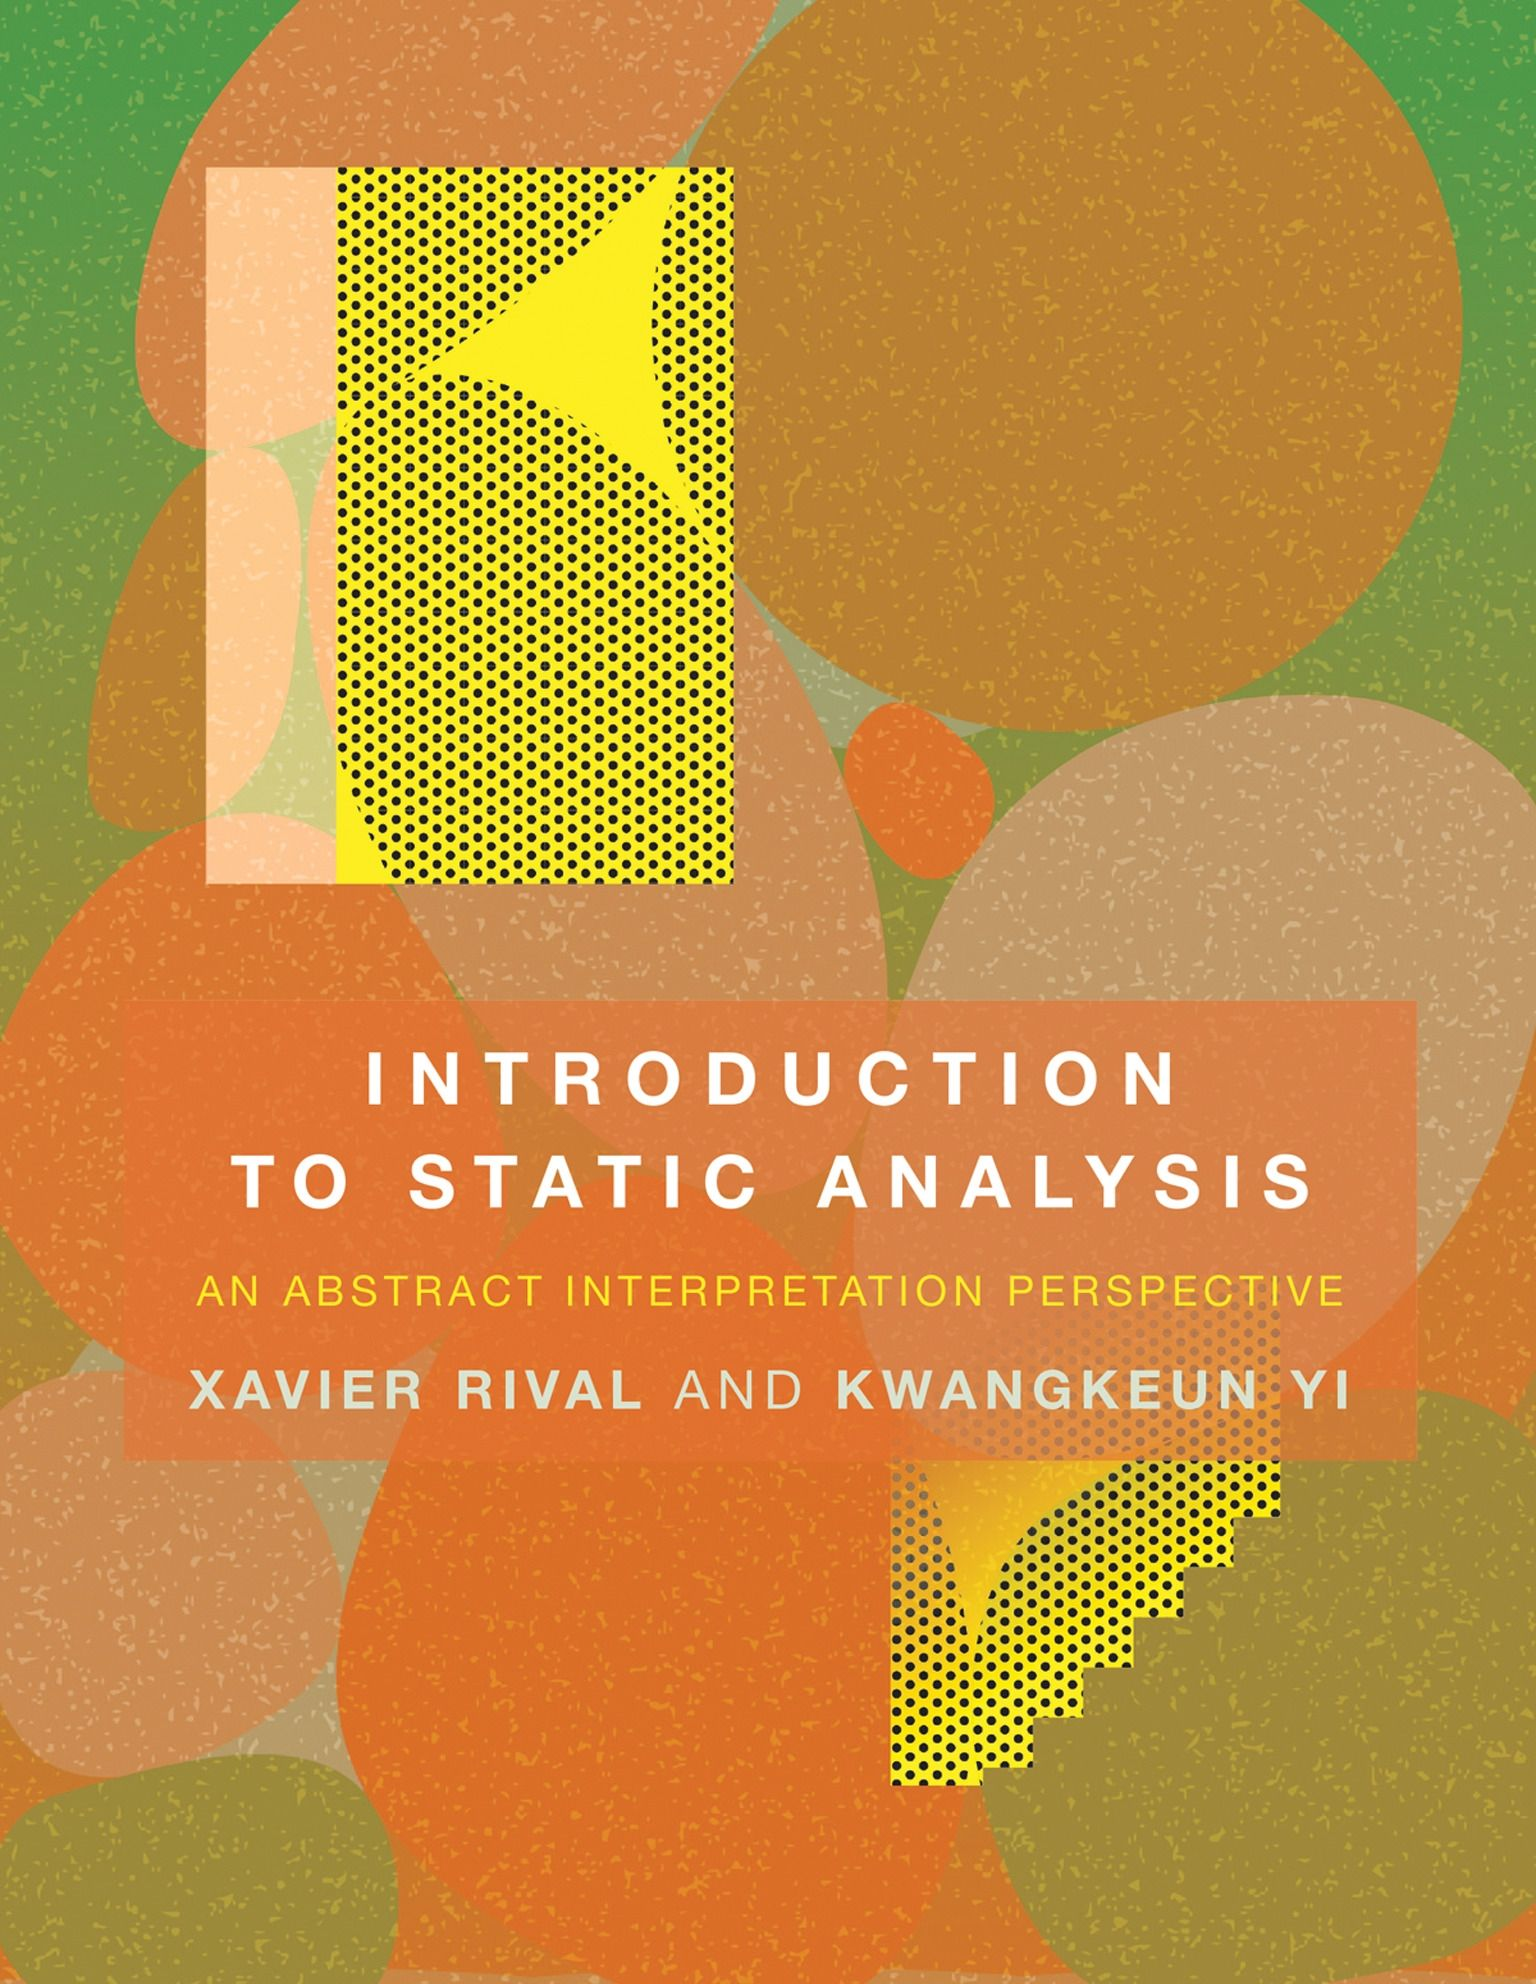
\includegraphics[width=4cm]{itsa-cover.jpg}}] (0,0) rectangle ++(3.8,5);
      \node[above] at(current bounding box.north) {\clap{\small\strut Using Analyses~\cite{rival2020introduction}}};
   }
\end{tikzpicture}}\hfill\raisebox{\dimexpr-\height+1cm}{\begin{tikzpicture}
   \onslide<3->{%
      \draw[darkgray,thick,rounded corners=2pt,path image={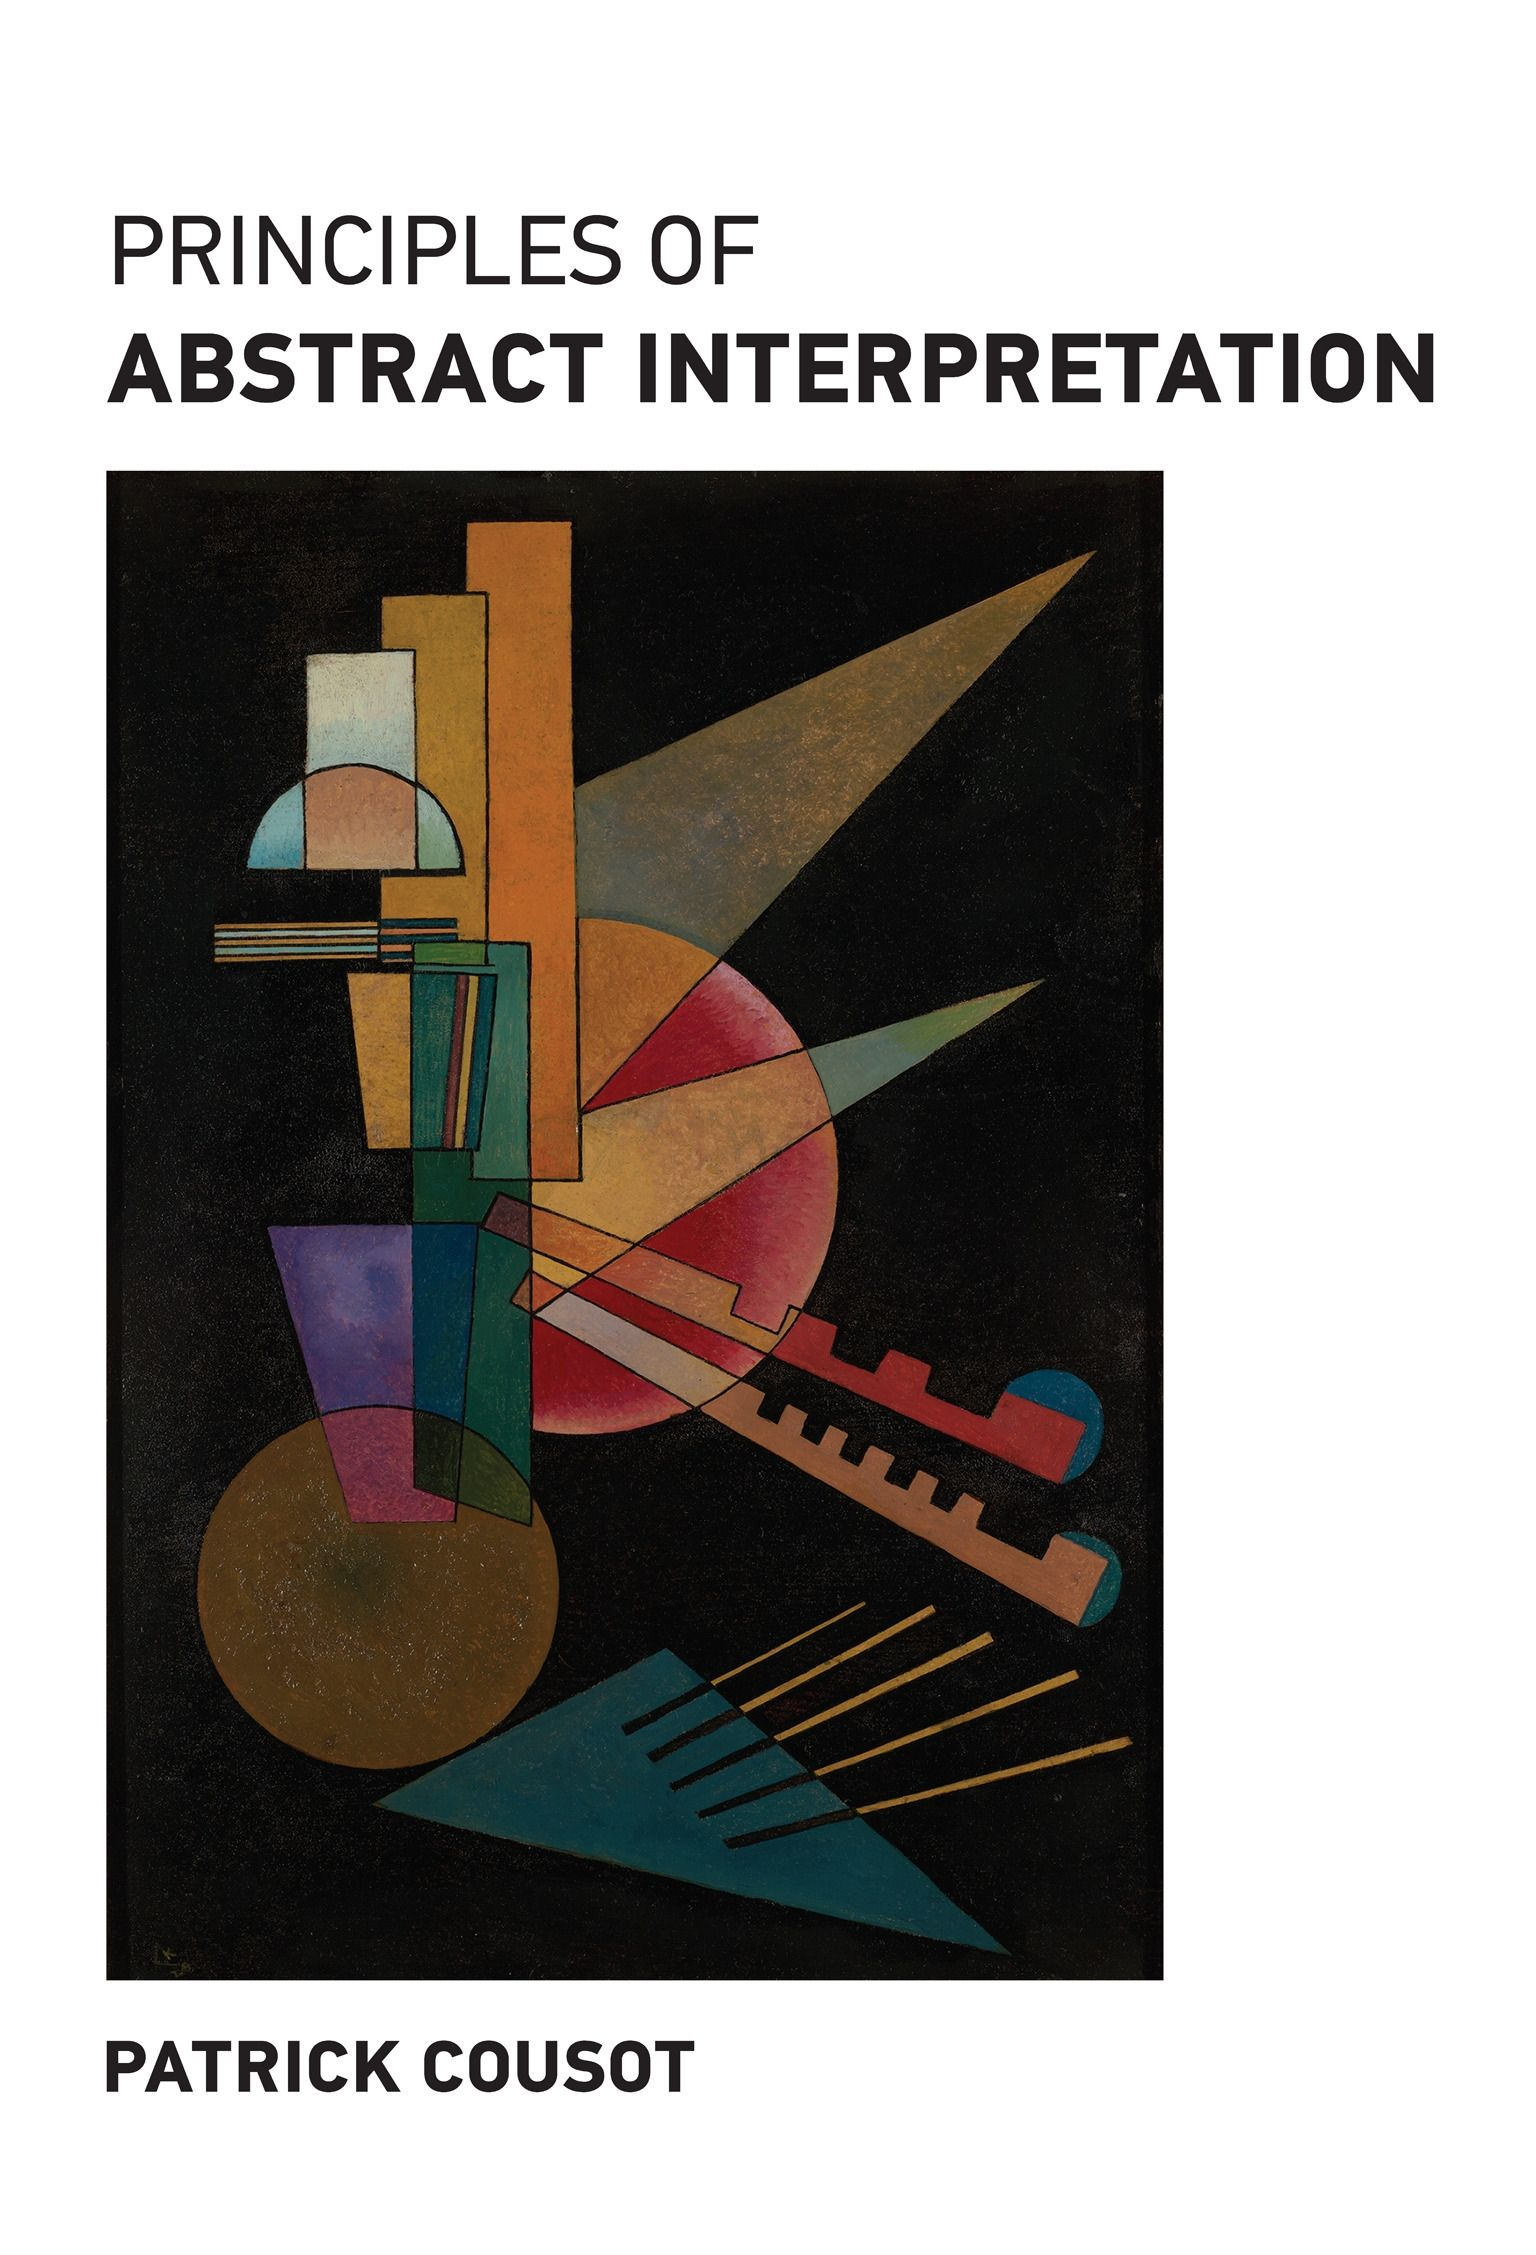
\includegraphics[width=4cm]{poa-cover.jpg}}] (0,0) rectangle ++(3.9,5.5);
      \node[above] at(current bounding box.north) {\clap{\small\strut Formal Foundations~\cite{cousout2021principles}}};
   }
\end{tikzpicture}}\hfill\raisebox{\dimexpr-\height+1cm}{\begin{tikzpicture}
   \onslide<4->{%
      \draw[darkgray,thick,rounded corners=2pt,path image={
\includegraphics[width=4cm]{dfa-cover.jpg}}] (0,0) rectangle ++(3.9,6);
      \node[above] at(current bounding box.north) {\clap{\small\strut Dataflow Perspective~\cite{rival2020introduction}}};
   }
\end{tikzpicture}}\hfill\strut
\begin{tikzpicture}[overlay,remember picture]
   \node[above right=0.5mm,yshift=3mm,gray,font=\tiny] at (current page.south west) {And for an overview: \citetitle{DBLP:journals/ftpl/Mine17}~\cite{DBLP:journals/ftpl/Mine17}};
\end{tikzpicture}
\end{frame}

\section{The How}

\begin{frame}[fragile]{Abstract Interpretation}
\begin{uncoverenv}<2->
\AnimateCode{onslide={o2:{3,...,7},-,-,-},first slide=2}
\begin{minted}[escapeinside=||,lineskip=1pt]{java}
public static void main(String[] args) {
    int a = 1; |\tikzmarknode{mark@a1}{\strut}|
    double r = Math.random() * 10; |\tikzmarknode{mark@r1}{\strut}|
    if (r > 5) { |\tikzmarknode{mark@r2}{\strut}|
       a = 2; |\tikzmarknode{mark@a2}{\strut}|
    }
    System.out.println(a); |\tikzmarknode{mark@a3}{\strut}|
}
\end{minted}
\endAnimateCode
\begin{tikzpicture}[overlay,remember picture]
   \coordinate (mark@a1) at (pic cs:mark@a1);
   \node[right=4cm,yshift=2.5pt] (mark@a1) at (mark@a1) {\AbstractInfo{a \in \Set{1}}};
   \coordinate (mark@r1) at (pic cs:mark@r1);
   \node[right,yshift=2.5pt] at (mark@r1-|mark@a1.west) {\AbstractInfo{r \in \IntCO{0}{10}}};
   \coordinate (mark@a2) at (pic cs:mark@a2);
   \node[right,yshift=2.5pt] at (mark@a2-|mark@a1.west) {\AbstractInfo{a \in \Set{2}}};
   \coordinate (mark@a3) at (pic cs:mark@a3);
   \node[right,yshift=2.5pt] (mark@set) at (mark@a3-|mark@a1.west) {\AbstractInfo{a \in \Set{1, 2}}};
   \node[right] at (mark@set.east) {\(\to\)~\;Valid? Ok? Safe?};
   \onslide<3->{%
      \fill[white,opacity=0.9] ([yshift=2cm]current page.west) rectangle ([yshift=-2cm]current page.east);
      \node[text width=.8\paperwidth,align=left] at(current page.center) {\begin{itemize}
         \itemsep10pt
         \item<4-> We want to proof interesting properties of programs
         \begin{itemize}
            \itemsep5pt
            \item<5-> \textit{Dataflow Properties}\\Liveness, Fainting, Reaching Definitions,~\ldots
            \item<6-> \textit{Safety Properties}\\No Null Dereference, No Division by Zero,~\ldots % finite prefix if we find violation
            \item<7-> \textit{Numerical Properties}\\Signs, Intervals, Octagons, Polyhedra,~\ldots
            \item<8-> \ldots
         \end{itemize}
      \end{itemize}};
   }%
   \node[above right,gray,yshift=3.5mm,font=\tiny,text width=.9\paperwidth] at (current page.south west) {\citetitle{cousout2021principles}~\cite[p.~722]{cousout2021principles},\citetitle{DBLP:journals/annals/GiacobazziR22}~\cite[pp.~37]{DBLP:journals/annals/GiacobazziR22}};
\end{tikzpicture}
\end{uncoverenv}
\end{frame}


\subsection{Terminology}

\newsavebox\GraphHeaven
\begin{frame}[c]{Abstract \textcolor{gray}{Interpretation}}
\frametitle<1>{Abstract \textcolor{gray}{Interpretation}}
\frametitle<2-|handout:1>{Concrete \textcolor{gray}{Interpretation}}
\frametitle<11-|handout:1>{Abstract \textcolor{gray}{Interpretation}}
% häufige Visualisierung
\begin{lrbox}{\GraphHeaven}
\pgfmathsetseed{42}%
\begin{tikzpicture}[line cap=round]
   \pgfonlayer{foreground}
   \draw[Kite-Kite,very thick] (0,3.5) node[below right,yshift=1mm] {{\onslide<3->{\(x(t)\)}}} |- (8,0) node[above left] {{\onslide<2->{\(t\)}}}; % time vs. x at tat time
   \endpgfonlayer
   \colorlet{@}{red}
   \onslide<4->{\only<5->{\colorlet{@}{gray}}\draw[very thick,@] (0,1) plot [smooth] coordinates {(0,1) (1,2) (2,1) (3,2) (4,1) (5,2) (6,1) (7,2) (8,1)}; % x(t)
   }
   \colorlet{@}{red}
   \onslide<5->{\only<6->{\colorlet{@}{gray}}\draw[very thick,@] (0,0) plot [smooth] coordinates {(0,0) (1,1) (2,2) (3,2) (4,2.5) (5,2.5) (6,.5) (7,.6) (8,.6)}; % x(t)
   }
   \colorlet{@}{red}
   \onslide<6->{\only<7->{\colorlet{@}{gray}}\draw[very thick,@] (0,1.5) plot [smooth] coordinates {(0,1.5) (1,2) (2,2.5) (3,2) (4,2) (5,2.5) (6,2.5) (7,2) (8,2.5)}; % x(t)
   }
   \onslide<8->{
      \foreach \i in {0,...,5} {
         \pgfmathsetmacro{\randA}{rnd*0.33}
         \pgfmathsetmacro{\randB}{rand*0.5}
         \pgfmathsetmacro{\randC}{rand*0.4}
         \draw[gray] (0,1.5+\randA) plot [smooth] coordinates {(0,1.5+\randA) (1,2-\randB) (2,2.5-\randA) (3,2-\randB) (4,2+\randA) (5,2.5) (6,2.5+\randA) (7,2-\randA) (8,2.5+\randB)} node[inner sep=0pt] (a-\i) {};
         \draw[gray] (0,0+\randA) plot [smooth] coordinates {(0,0+\randA) (1,1-\randB) (2,2-\randB) (3,2+\randC) (4,2.5-\randA) (5,2.5-\randB) (6,.5+\randC) (7,.6+\randB) (8,.6+\randC)} node[inner sep=0pt] (b-\i) {};
         \draw[gray] (0,1+\randB) plot [smooth] coordinates {(0,1-\randC) (1,2-\randB) (2,1+\randB) (3,2-\randA) (4,1+\randA) (5,2-\randB) (6,1) (7,2-\randC) (8,1+\randA)} node[inner sep=0pt] (c-\i) {};
      }
   }
   % fit to all nodes to get the bounding box
   \node[fit=(a-0) (a-1) (a-2) (a-3) (a-4) (a-5) (b-0) (b-1) (b-2) (b-3) (b-4) (b-5) (c-0) (c-1) (c-2) (c-3) (c-4) (c-5),inner sep=0pt] (big-ghost) {~};
   \onslide<9->{
      \draw[decorate,thick,decoration={brace,amplitude=5pt,raise=2pt},gray] (big-ghost.north east) -- (big-ghost.south east) node[midway,right=7pt,gray,align=left] (@doc) {Collecting Semantics\textsuperscript{\cite[91]{cousout2021principles}}};
   }
   \onslide<10->{
      \node[below right,xshift=-2mm,yshift=5mm,font=\footnotesize,text width=6cm,opacity=.5] at (@doc.south west) {\begin{itemize}
         \itemsep-1pt
         \item Maybe impossible to compute statically
         \item \ldots~or very expensive (\faCaretRight~\textit{dynamic})
         \item[\faCaretRight] Abstract Interpretation to the rescue
      \end{itemize}};
   }
   \pgfonlayer{background}
   \only<11|handout:0>{
   \fill[red,opacity=.175,even odd rule] plot [smooth] coordinates {(0,0) (1,0.4) (2,0.5) (3,1) (4,.8) (5,1) (6,.1) (7,0.2) (8.03,.2) (8.03,3) (7,2.8) (6,3) (5,2.95) (4,2.85) (3,2.75) (2,2.65) (1,2.5) (0,2) } -- cycle; 
   }
   \only<12->{
   \fill[red,opacity=.175,even odd rule] plot [smooth] coordinates {(0,0) (1,0.4) (2,0.5) (3,1) (4,.8) (5,1) (6,.1) (7,0.2) (8.03,.2) (8.03,3) (7,2.8) (6,3) (5,2.95) (4,2.85) (3,2.75) (2,2.65) (1,2.5) (0,2) } -- cycle (6,1.85) circle[radius=4mm]; 
   }
   \onslide<11->{%
      \draw[Circle-,red,rounded corners=4pt] (7.75,2.9) -- ++(.35,.5) -- ++(.5,0) node[right,align=left] {(Trace) Abstraction\textsuperscript{\cite[92]{cousout2021principles}}\\[-2pt]\footnotesize\color{gray}just one of many};
   }
   \onslide<13->{
      \node (@b1) at (6,1.85) {\small\faBug};
      \node (@b2) at (3,.35) {\small\faBug};
      \node (@b3) at (7,2.5) {\small\faBug};
   }
   \onslide<14->{
      \node[above left=-1mm,green] at(@b2.south east) {\scriptsize\faCheck};
   }
   \onslide<15->{
      \node[above left=-1mm,green] at(@b1.south east) {\scriptsize\faCheck};
   }
   \onslide<16->{
      \node[above left=-1mm,yshift=1pt,orange] at(@b3.south east) {\scriptsize\faQuestion};
   }
   \endpgfonlayer
   \path[use as bounding box] (0,0) rectangle (8,3.5);
\end{tikzpicture}
\end{lrbox}
\begin{tikzpicture}[overlay,remember picture]
   \node[xshift=2.5mm] at(current page.center) {\usebox\GraphHeaven};
   \node[above right,gray,yshift=3.5mm,font=\tiny,text width=.9\paperwidth] at (current page.south west) {See \citetitle{cousout2012casual}~\cite{cousout2012casual}};
\end{tikzpicture}
\end{frame}
\newsavebox\PowersetZHasse
\newsavebox\TestBox
% TOOD: measure and only box if larger?
\begin{lrbox}{\PowersetZHasse}
\def\S#1{\savebox\TestBox{\footnotesize\absexpr{\Set{#1}}}\ifdim\ht\TestBox>5mm\makebox[5mm][c]{\usebox\TestBox}\else\usebox\TestBox\fi}\color{gray}%
\begin{tikzpicture}
   \matrix (A) [matrix of nodes, row sep=1mm, column sep=-2mm]
   {
       & & & \kern-4mm\S{-4, 0, 1, 9}\kern-4mm & & & \\
       & & \S{-4,0,1} & \ldots & \S{0,1,9} & & \\
      & \S{-4,0} & \ldots & \S{0,1} & \ldots & \S{1,9} & \\
      \S{-4} & \ldots & \S{0} & \ldots & \S{1} & \ldots & \S{9} \\
      & & & \absexpr{\emptyset} & & & \\
   };
   \scope[line cap=round]
   \draw (A-1-4) -- (A-2-3) -- (A-3-2) -- (A-4-1) (A-4-1.south) -- (A-5-4);
   \draw (A-1-4) -- (A-2-5) -- (A-3-6) -- (A-4-7) (A-4-7.south) -- (A-5-4);
   \draw (A-3-2) -- (A-4-3) -- (A-3-4) (A-3-4) -- (A-4-5) -- (A-3-6);
   \draw (A-2-3) -- (A-3-4) -- (A-2-5);
   \draw (A-4-3) -- (A-5-4) -- (A-4-5);
   \draw[densely dotted] (A-5-4) -- ++(-1,0.05)  (A-5-4) -- ++(1,0.05);
   \foreach[count=\y] \i in {4,3,2,1} {
      \draw[densely dotted] (A-\y-\i.north west) -- ++(-.4,0.14);
      \node[left=3.5mm] at(A-\y-\i.west) {\footnotesize\ldots};
      \pgfmathsetmacro\other{int(8-\i)}
      \draw[densely dotted] (A-\y-\other.north east) -- ++(.4,0.14);
      \node[right=3.5mm] at(A-\y-\other.east) {\footnotesize\ldots};
   }
   \node[above=3.5mm] (pz) at(A-1-4.north) {\absexpr{\P(\Z)}};
   \draw[densely dotted] (pz) -- ++(-1.25,-0.1) (pz) -- ++(1.25,-0.1);
   \draw[-Kite] ([yshift=1cm,xshift=-3mm]current bounding box.south west) -- ([yshift=-5mm]current bounding box.north west) node[midway,left,font=\scriptsize] {\rotatebox{90}{\absexpr{\partof \asdef\eq \subseteq}}};
   \endscope
\end{tikzpicture}
\end{lrbox}
\begin{frame}{Terminology}
   \begin{itemize}
      \item \textsb{Property}\onslide<2->{ --- Set of states/traces that satisfy that property}\\
            \onslide<3->{\textcolor{gray}{Even integers: \absexpr{\text{P} = \Set{ z \in \Z \Given \exists k \in \Z : z = 2k} = \Set{0, 2, 4, 6, \ldots} \subseteq \P(\tikzmarknode{universe}{\Z})}}}
            \medskip

            \onslide<5->{\centerline{\absexpr{\tikzmarknode{ff}{\emptyset} \subseteq \tikzmarknode{p1}{\text{P}_1} \subseteq \tikzmarknode{p2}{\text{P}_2} \subseteq \tikzmarknode{tt}{\Universe}}}}
            \vspace*{4.9em}

      \item<10-> \textsb{Partial Order} \onslide<11->{--- A \tikzmarknode{reflexive}{reflexive}, \tikzmarknode{transitive}{transitive}, \tikzmarknode{antisymmetric}{antisymmetric} relation on a set}\\
            \textcolor{gray}{\onslide<15->{\absexpr{(\Z, \leq)}}\onslide<16->{,\quad\absexpr{(\P(\Z), \subseteq)},\quad\ldots}}
            % domains special kinds of partial orders
   \end{itemize}
   
   \begin{tikzpicture}[overlay,remember picture,line cap=round]
      \onslide<4->{
         \draw[Kite-,gray] ([yshift=-2pt]universe.south) to[out=310,in=180] ++(.4,-.25) node[right] {\small universe (\absexpr{\Universe})};
      }
      \onslide<6->{\draw[Kite-,gray] ([yshift=-2pt]ff.south) to[out=230,in=0] ++(-.4,-.25) node[left] {\small strongest};}
      \onslide<7->{\draw[Kite-,gray] ([yshift=-2pt,xshift=-2pt]p1.south) to[out=260,in=0] ++(-.4,-.55) node[left] {\small stronger};}
      \onslide<8->{\draw[Kite-,gray] ([yshift=-2pt,xshift=-2pt]p2.south) to[out=280,in=180] ++(.4,-.55) node[right] {\small weaker};}
      \onslide<9->{\draw[Kite-,gray] ([yshift=-2pt]tt.south) to[out=310,in=180] ++(.4,-.25) node[right] {\small weakest};}
      
      \onslide<12->{\draw[Kite-,gray] ([yshift=2pt]reflexive.north) to[out=130,in=0] ++(-.4,.215) node[left] {\small \absexpr{\forall x \in X : x \partof x}};}
      \onslide<13->{\draw[Kite-,gray] ([yshift=2pt]transitive.north) -- ++(0,.3) node[above=-1pt] {\small \absexpr{\forall x, y, z \in X : x \partof y \land y \partof z \implies x \partof z}};}
      \onslide<14->{\draw[Kite-,gray] ([yshift=2pt]antisymmetric.north) to[out=50,in=180] ++(.4,.215) node[right] {\kern-1pt\small\absexpr{\forall x, y \in X : x \partof y \land y \partof x \implies x = y}};}
      
      \node[above right,gray,yshift=3.5mm,font=\tiny,text width=.9\paperwidth] at (current page.south west) {\citetitle{cousout2021principles}~\cite[15]{cousout2021principles},\citetitle{DBLP:journals/ftpl/Mine17}~\cite[18]{DBLP:journals/ftpl/Mine17}};
      \onslide<17->{%
      \node[above left,yshift=3.5mm] at(current page.south east) {\scalebox{.65}{\usebox\PowersetZHasse}};
      }
   \end{tikzpicture}
\end{frame}

\def\S#1{\savebox\TestBox{\footnotesize\absexpr{\Set{#1}}}\ifdim\ht\TestBox>5mm\makebox[5mm][c]{\usebox\TestBox}\else\usebox\TestBox\fi}%
\def\I#1#2{\footnotesize\absexpr{\IntCC{#1}{#2}}}
\begin{frame}[fragile]{Chains and Lattices}
\begin{onlyenv}<1|handout:0>
\begin{tikzpicture}
   \matrix (A) [matrix of nodes, row sep=2.5mm, column sep=-2mm]
   {
       & &  & \kern-4mm\S{-4, 0, 1, 9}\kern-4mm & & & \\
       & & \S{-4,0,1} & \ldots & \S{0,1,9} & & \\
      & \S{-4,0} & \ldots & \S{0,1} & \ldots & \S{1,9} & \\
      \S{-4} & \ldots & \S{0} & \ldots & \S{1} & \ldots & \S{9} \\
      & & & \absexpr{\emptyset} & & & \\
   };
   \scope[line cap=round]
   \draw (A-1-4) -- (A-2-3) -- (A-3-2) -- (A-4-1) (A-4-1.south) -- (A-5-4);
   \draw (A-1-4) -- (A-2-5) -- (A-3-6) -- (A-4-7) (A-4-7.south) -- (A-5-4);
   \draw (A-3-2) -- (A-4-3) -- (A-3-4) (A-3-4) -- (A-4-5) -- (A-3-6);
   \draw (A-2-3) -- (A-3-4) -- (A-2-5);
   \draw (A-4-3) -- (A-5-4) -- (A-4-5);
   \draw[densely dotted] (A-5-4) -- ++(-1,0.05)  (A-5-4) -- ++(1,0.05);
   \foreach[count=\y] \i in {4,3,2,1} {
      \draw[densely dotted] (A-\y-\i.north west) -- ++(-.4,0.14);
      \node[left=3.5mm] at(A-\y-\i.west) {\footnotesize\ldots};
      \pgfmathsetmacro\other{int(8-\i)}
      \draw[densely dotted] (A-\y-\other.north east) -- ++(.4,0.14);
      \node[right=3.5mm] at(A-\y-\other.east) {\footnotesize\ldots};
   }
   \node[above=3.5mm] (pz) at(A-1-4.north) {\absexpr{\P(\Z)}};
   \draw[densely dotted] (pz) -- ++(-1.25,-0.1) (pz) -- ++(1.25,-0.1);
   \draw[-Kite] ([yshift=1cm,xshift=-3mm]current bounding box.south west) -- ([yshift=-5mm]current bounding box.north west) node[midway,left,font=\scriptsize] {\rotatebox{90}{\absexpr{\partof \asdef\eq \subseteq}}};
   \endscope
\end{tikzpicture}
\end{onlyenv}
\begin{onlyenv}<2-|handout:1>
\begin{tikzpicture}
   \matrix (A) [matrix of nodes, row sep=2.5mm, column sep=-2mm]
   {
       & &  & \I{-1}{\infty} & & & \\
       & & \I{-1}{1} & \ldots & \I{0}{9} & & \\
      & \I{-1}{0} & \ldots & \I{0}{1} & \ldots & \I{1}{9} & \\
      \I{-1}{-1} & \ldots & \I00 & \ldots & \I11 & \ldots & \I99 \\
      & & & \absexpr{\bot} & & & \\
   };
   \scope[line cap=round]
   \draw (A-2-3) -- (A-3-2) -- (A-4-1) -- (A-5-4);
   \draw (A-3-6) -- (A-4-7) -- (A-5-4);
   \draw (A-3-2) -- (A-4-3) -- (A-3-4) (A-3-4) -- (A-4-5) -- (A-3-6);
   \draw (A-2-3) -- (A-3-4);
   \draw (A-4-3) -- (A-5-4) -- (A-4-5);
   \draw[densely dotted] (A-2-5) -- (A-1-4) -- (A-2-3) (A-3-4) -- (A-2-5) -- (A-3-6);
   \draw[densely dotted] (A-5-4) -- ++(-1,0.05)  (A-5-4) -- ++(1,0.05);
   \foreach[count=\y] \i in {4,3,2,1} {
      \draw[densely dotted] (A-\y-\i.north west) -- ++(-.4,0.14);
      \node[left=3.5mm] at(A-\y-\i.west) {\footnotesize\ldots};
      \pgfmathsetmacro\other{int(8-\i)}
      \draw[densely dotted] (A-\y-\other.north east) -- ++(.4,0.14);
      \node[right=3.5mm] at(A-\y-\other.east) {\footnotesize\ldots};
   }
   \node[above=3.5mm] (pz) at(A-1-4.north) {\absexpr{\top}};
   \draw[densely dotted] (pz) -- ++(-1.25,-0.1) (pz) -- ++(1.25,-0.1);
   \draw[-Kite] ([yshift=1cm,xshift=-3mm]current bounding box.south west) -- ([yshift=-5mm]current bounding box.north west) node[midway,left,font=\scriptsize] {\rotatebox{90}{\absexpr{\partof \asdef\eq \dot\subseteq}}};
   \endscope
   \pgfonlayer{background}
   \scope[opacity=.175,transparency group]
   \onslide<6->{%
      \draw[red,line width=3mm,rounded corners=2mm,line cap=round] (pz.center) -- ++(1.25,-.42) coordinate (@edge) -- (A-1-4.center) -- (A-2-3.center) -- (A-3-2.center) -- (A-4-1.center) -- (A-5-4.center);
      \foreach \i in {pz,A-1-4,A-2-3,A-3-2,A-4-1,A-5-4} {
         \fill[red,rounded corners=5pt,line cap=round] (\i.south west) rectangle (\i.north east);
      }
   }
   \endscope
   \onslide<4->{
      \draw[Kite-,red,rounded corners=4pt] ([xshift=1.5mm,yshift=-1mm]A-3-4.north) -- ++(.25,.325) -- ++(3,0) node[below right,yshift=.7\baselineskip,align=left] {Least upper bound\\[-2pt]\footnotesize\color{gray}of \IntCC00 and \IntCC11\\[-3pt]\footnotesize\color{gray}lub, join, \absexpr{\lub}};
   }
   \onslide<5->{
      \draw[Kite-,red,rounded corners=4pt] ([xshift=1mm,yshift=1mm]A-4-3.south) -- ++(-.4,-.85) -- ++(-.25,0) node[below left,yshift=.7\baselineskip,align=right] {Greatest lower bound\\[-2pt]\footnotesize\color{gray}of \IntCC{-1}{0} and \IntCC01\\[-3pt]\footnotesize\color{gray}glb, meet, \absexpr{\glb}};
   }
   \onslide<6->{
      \draw[Circle-,red,rounded corners=4pt] ([xshift=-1mm]@edge) -- ++(.35,.5) -- ++(.5,0) node[below right,yshift=.7\baselineskip,align=left] {Chain\\[-2pt]\footnotesize\color{gray}a totally ordered subset\\[-4pt]{\footnotesize\color{gray}\onslide<7->{e.g., \absexpr{\IntCC{0}{0} \partof \IntCC{0}{9} \partof \IntCC{-10}{200}}}}};
   }
   \endpgfonlayer
   \pgfinterruptboundingbox
   \onslide<3->{%
      \draw[Kite-,gray] (A-5-4.south) to[out=-60,in=180] ++(.5,-.25) node[right,font=\scriptsize] {bottom, empty interval};
      \draw[Kite-,gray] (pz.north) to[out=120,in=0] ++(-.5,.25) node[left,font=\scriptsize] {top, \absexpr{\IntCC{-\infty}{\infty}}};
   }
   \endpgfinterruptboundingbox
\end{tikzpicture}
\begin{tikzpicture}[overlay,remember picture]
\onslide<8->{%
   \node[above left,yshift=4.345mm,text width=5.5cm] at(current page.south east) {\textsb{Complete Lattice} \absexpr{(X, \partof, \lub, \glb, \bot, \top)}\vspace{-3.5mm}\footnotesize
   {\begin{itemize} 
      \itemsep-1pt
      \item<9-> \absexpr{(X, \partof)} is a partial order
      \item<10-> \absexpr{\forall A \subseteq X : \lub A} and \absexpr{\glb A} exist
      \item<11-> \absexpr{\bot}/\absexpr{\top} as smallest/largest element
   \end{itemize}}
   };
}
\end{tikzpicture}
\end{onlyenv}
% birkhoff1940lattice
\begin{tikzpicture}[overlay,remember picture]
   \node[above right,gray,yshift=3.5mm,font=\tiny,text width=.9\paperwidth] at (current page.south west) {\citetitle{birkhoff1967lattice}~\cite{birkhoff1967lattice}, see also sublattices~\cite[25]{DBLP:journals/ftpl/Mine17}};
\end{tikzpicture}
\end{frame}

\subsection{Abstract Domains}
\begin{frame}{\insertsubsection~\qquad\textcolor{gray}{Numerical}}
\vspace*{3.5em}
\tikzset{@/.style={red}}\only<5->{\tikzset{@/.style={gray}}}%
\begin{tikzpicture}[line cap=round]
   \draw[-Kite] (0,-1) -- (0,1) node[below left] {\scriptsize y};
   \draw[-Kite] (-1,0) -- (1,0) node[below left] {\scriptsize x};
\scope[@]
\onslide<2->{%
   \fill (.1,.1) coordinate (@) circle[radius=1.5pt];
   \foreach \x/\y in {.2/.3,-.1/.2,-.3/-.2,.2/-.5,.5/.4,-.8/.7,-.9/-.4,.4/.4,.35/-.4,-.4/.3} {
      \fill (\x,\y) circle[radius=1.5pt];
      \draw[-{Kite[scale=.4]}] (@) -- (\x,\y) coordinate (@);
   }
}
\onslide<3->{%
   \fill (-.4,-.55) circle[radius=1.5pt];
   \fill (.5,-.8) circle[radius=1.5pt];
   \draw[-{Kite[scale=.4]}] (-.4,-.55) -- (.5,-.8);
}
\endscope
\onslide<4->{%
   \node[below=1mm] at(current bounding box.south) {\scriptsize Collecting Semantics};
}
\end{tikzpicture}\hfill\onslide<5->{%
\tikzset{@/.style={red}}\only<8->{\tikzset{@/.style={gray}}}%
\begin{tikzpicture}[line cap=round]
   \draw[-Kite] (0,-1) -- (0,1) node[below left] {\scriptsize y};
   \draw[-Kite] (-1,0) -- (1,0) node[below left] {\scriptsize x};
\pgfonlayer{background}
\scope[@]
\onslide<6->{%
   \fill[@,opacity=.4] (-.4,-1) rectangle (.7,1);
   \draw[gray,thin] (-.4,-1) -- ++(0,2);
   \draw[gray,thin] (.7,-1) -- ++(0,2);
}
\endscope
\endpgfonlayer
\onslide<7->{%
   \node[below=1mm] at(current bounding box.south) {\clap{\scriptsize Intervals \absexpr{x \in \IntCC ab}}};
}
\end{tikzpicture}}\hfill\onslide<9->{%
\tikzset{@/.style={red}}\only<11->{\tikzset{@/.style={gray}}}%
\begin{tikzpicture}[line cap=round]
   \draw[-Kite] (0,-1) -- (0,1) node[below left] {\scriptsize y};
   \draw[-Kite] (-1,0) -- (1,0) node[below left] {\scriptsize x};
\scope[@]
\onslide<10->{%
   \foreach \x in {-1,-.7,...,1} {
      \foreach \y in {-.9,-.6,...,1} {
         \fill (\x,\y) circle[radius=1.5pt];
      }
   }
}
\endscope
\onslide<10->{%
   \node[below=1mm] at(current bounding box.south) {\clap{\scriptsize Simple Congruences}};
}
\end{tikzpicture}}\hfill\onslide<11->{%
\tikzset{@/.style={red}}\only<13->{\tikzset{@/.style={gray}}}%
\begin{tikzpicture}[line cap=round]
   \draw[-Kite] (0,-1) -- (0,1) node[below left] {\scriptsize y};
   \draw[-Kite] (-1,0) -- (1,0) node[below left] {\scriptsize x};
\scope[@]
\onslide<12->{%
   \fill[opacity=.4,@] (-.5,-.3) |- ++(.8,.6) -- ++(0,-.4) -- ++(-.2,-.2) -- cycle;
   \draw[gray,thin] (-.5,-.3) |- ++(.8,.6) -- ++(0,-.4) -- ++(-.2,-.2) -- cycle;
   \draw[thick,@] (.6,.2) -- ++(-.8,-.8);
}
\endscope
\onslide<12->{%
   \node[below=1mm] at(current bounding box.south) {\clap{\scriptsize Pentagons}};
}
\end{tikzpicture}}
\medskip
\begin{multicols}{4}
\begin{itemize}
   \item<14-> Octagons
   \item<15-> Ellipses
   \item<16-> Exponentials
   \item<17-> Signs
\end{itemize}
\end{multicols}
\begin{tikzpicture}[overlay,remember picture]
   \node[above right,gray,yshift=3.5mm,font=\tiny,text width=.9\paperwidth] at (current page.south west) {\citetitle{cousout2021principles}~\cite{cousout2021principles}, \citetitle{DBLP:conf/sac/LogozzoF08}~\cite[25]{DBLP:conf/sac/LogozzoF08}};
\end{tikzpicture}
% non relational: pointer, shapes, cost, ...
\end{frame}

\subsection{Sign Analysis}
\newsavebox\SimpleSignLattice
\begin{lrbox}{\SimpleSignLattice}
\scriptsize
\begin{tikzpicture}[line cap=round,x=6.5mm,y=6.5mm]
   \node (top) at (0,0) {\absexpr{\top}};
   \node (pos) at (-1,-1) {\absexpr{\geq 0}};
   \node (neg) at (1,-1) {\absexpr{\leq 0}};
   \node (zero) at (0,-2) {\absexpr{0}};
   \node (bot) at (0,-3) {\absexpr{\bot}};
   \draw (top) -- (pos) -- (zero) -- (neg) -- (top) (zero) -- (bot);
\end{tikzpicture}
\end{lrbox}
\begin{frame}[fragile]{\insertsubsection\hfill\textcolor{gray}{Simple Sign Domain}}
\begin{itemize}
   \item<3-> We still have no program semantics, but we can try\ldots
\begin{minted}[escapeinside=||,lineskip=1pt]{java}
int a = 0; |\tikzmark{n@a1}|
int b = 12; |\tikzmark{n@b1}|
int c = a + b; |\tikzmark{n@c1}|
int d = c - b; |\tikzmark{n@d1}|
\end{minted}
\begin{tikzpicture}[overlay,remember picture]
   \onslide<4->{%
      \coordinate (n@a1) at (pic cs:n@a1);
      \node[right=2cm] (n@a1) at (n@a1) {\AbstractInfo{a = 0}};
   }%
   \onslide<5->{%
      \coordinate (n@b1) at (pic cs:n@b1);
      \node[right] at (n@b1-|n@a1.west) {\AbstractInfo{b \geq 0}};
   }%
   \onslide<6->{%
      \coordinate (n@c1) at (pic cs:n@c1);
      \node[right] at (n@c1-|n@a1.west) {\AbstractInfo{c \geq 0\quad (={} 0~{}+{}\geq 0)}};
   }%
   \onslide<7->{%
      \coordinate (n@d1) at (pic cs:n@d1);
      \node[right] (n@d1) at (n@d1-|n@a1.west) {\AbstractInfo{d = \top\kern-1.5pt\quad (\geq{} 0~{}-{}\geq 0)}};
   }
\end{tikzpicture}
   \item<8-> But how to handle control flow? Loops? Recursion?
\end{itemize}

\begin{tikzpicture}[overlay,remember picture]
   \onslide<2->{\node[above left=.5mm,yshift=3.5mm] at(current page.south east) {\usebox\SimpleSignLattice};}
\end{tikzpicture}
\end{frame}


\subsection{Fixpoints}
\begin{frame}{\insertsubsection}
   \begin{itemize}
      \itemsep10pt
      \item<2-> For operators \(f: X \to X\) a \textsb{fixpoint} is a \(x \in X\) such that \(f(x) = x\)
      \item<3-> If we iterate \(f\) starting from some \(x_0 \in X\):\medskip
      \begin{itemize}[--]
         \itemsep15pt
         \item<4-> \parbox{3.25cm}{\smash{\tikz[baseline=-1.25mm,gray]{\coordinate (@) at (0,0);\fill (@) circle[radius=2pt] node[below] {\tiny\(x_0\)};\foreach \i in {0,...,3} {
            \draw[-Kite] (@) -- ++(.5,0) coordinate[xshift=1pt] (@);
            \fill (@) circle[radius=2pt] node[below] {\tiny\(f_\i\)};
         }; \draw[Kite-] ([xshift=-1pt]@) to[out=120,in=60,looseness=10] ([xshift=2pt]@);}}} \onslide<5->{reach a fixpoint, \(f^p = f(f^p)\)}
         \item<6-> \parbox{3.25cm}{\smash{\tikz[baseline=-1.25mm,gray]{\coordinate (@) at (0,0);\fill (@) circle[radius=2pt] node[below] {\tiny\(x_0\)};\foreach \i in {0,...,3} {
            \draw[-Kite] (@) -- ++(.5,0) coordinate[xshift=1pt] (@) coordinate (@\i);
            \fill (@) circle[radius=2pt] node[below] {\tiny\(f_\i\)};
         }; \draw[-Kite] (@) to[out=70,in=60] (@1);}}} \onslide<7->{reach a cycle, \(f^{p + \ell} = f^p, \ell > 0\)}
         \item<8-> \parbox{3.25cm}{\smash{\tikz[baseline=-1.25mm,gray]{\coordinate (@) at (0,0);\fill (@) circle[radius=2pt] node[below] {\tiny\(x_0\)};\foreach \i in {0,...,3} {
            \draw[-Kite] (@) -- ++(.5,0) coordinate[xshift=1pt] (@) coordinate (@\i);
            \fill (@) circle[radius=2pt] node[below] {\tiny\(f_\i\)};
         }; \draw[densely dotted] (@) -- ++(0.5,0)}}} \onslide<9->{iterate forever, \(\forall p \neq q : f^{p} \neq f^q\)}
      \end{itemize}
      \item<10-> If our function is monotonic, we can always find a fixpoint~\textsuperscript{\cite{tarski1955lattice}}
   \end{itemize}
\begin{tikzpicture}[overlay,remember picture]
   \node[above right,gray,yshift=3.5mm,font=\tiny,text width=.9\paperwidth] at (current page.south west) {\citetitle{tarski1955lattice}~\cite{tarski1955lattice}};
\end{tikzpicture}
\end{frame}

\section{Semantics}

\begin{frame}{\insertsection}
   
\end{frame}

\begin{frame}{Denotational Semantics}
   
\end{frame}

\subsection{Interval Analysis}
\begin{frame}{\insertsubsection}
   
\end{frame}

\section{Sound and Complete}
\begin{frame}{Soundness and Completeness}
   
\end{frame}

% \begin{frame}{Galois Connection}
   
% \end{frame}


\section{Domain Transformer}
\begin{frame}{\insertsection}
   
\end{frame}




% \begin{frame}
%                % TODO: hasse diagram for subseteq, then talk about lub and glb, chains, and what we want in the analysis

%    What is a Property? Set basis Poset etc. 
%    I have to abstract! 
%    Galois, Semantics Principles of Abstract Interpretation book
% \end{frame}

\begin{frame}[allowframebreaks]{References}
   \printbibliography
\end{frame}

\end{document}